\documentclass[12pt,border=4pt]{standalone}
\usepackage{fontspec}
\setmainfont{BeVietnamPro}[Path=D:/IOT_Tools/downloads/fonts/,Extension=.ttf,UprightFont=*-Regular,BoldFont=*-SemiBold]
\usepackage{amsmath}
\usepackage{unicode-math}\setmathfont{Cambria Math}
\usepackage[table]{xcolor}
\usepackage{tikz}
\usetikzlibrary{positioning,arrows.meta,shapes.geometric,calc,fit,backgrounds,decorations.pathreplacing,shadows}
\usepackage{tikz-3dplot}
\usepackage{pgfplots}\pgfplotsset{compat=1.18}
\usepgfplotslibrary{groupplots,fillbetween}
\definecolor{cXanh}{HTML}{1F5A96}\definecolor{cCam}{HTML}{E07B24}\definecolor{cLuc}{HTML}{2E8B57}
\definecolor{cHong}{HTML}{C2397F}\definecolor{cTim}{HTML}{6B4FA0}\definecolor{cXam}{HTML}{5B6770}\definecolor{cVang}{HTML}{D8A51D}
\pgfplotsset{baocao/.style={tick label style={font=\scriptsize}, scaled ticks=false, /pgf/number format/fixed,
  label style={font=\small}, legend style={font=\scriptsize,draw=none,fill=none},
  /pgf/number format/use comma, /pgf/number format/1000 sep={\,}, axis line style={cXam}, major tick style={cXam},
  ymajorgrids, grid style={cXam!20}}}
\pgfplotsset{colormap={baocao}{rgb255=(31,90,150) rgb255=(107,79,160) rgb255=(194,57,127) rgb255=(224,123,36) rgb255=(216,165,29)}}
\pgfkeys{/pgf/number format/assume math mode=true}
\newcommand{\ci}[2]{[#1;\,#2]}\newcommand{\so}[1]{#1}
\begin{document}
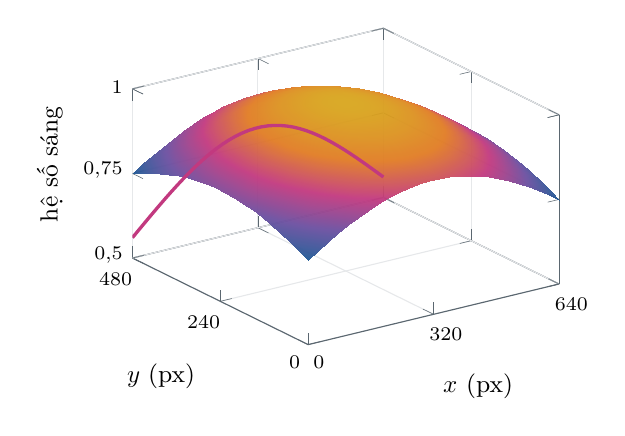
\begin{tikzpicture}
\begin{axis}[baocao, ymajorgrids=false, width=7.0cm, height=5.6cm, view={-35}{32},
  xlabel={$x$ (px)}, ylabel={$y$ (px)}, zlabel={hệ số sáng},
  xmin=0,xmax=640,ymin=0,ymax=480,zmin=0.5,zmax=1.0,
  xtick={0,320,640}, ytick={0,240,480}, ztick={0.5,0.75,1},
  /pgf/number format/precision=2,
  colormap name=baocao, grid=major, grid style={cXam!15}]
\addplot3[surf, shader=interp, samples=26, samples y=20, domain=0:640, y domain=0:480, opacity=0.95]
  {1/(1+((x-320)^2+(y-240)^2)/1016.1^2)^2};
\addplot3[cHong, line width=1.2pt, samples=40, domain=0:640, samples y=1]
  (x,480,{1/(1+((x-320)^2+240^2)/690^2)^2});
\end{axis}
\end{tikzpicture}
\end{document}
